\documentclass[a4paper, 12pt, twoside]{article}
\usepackage[T2A,T1]{fontenc}
\usepackage[utf8]{inputenc}
\usepackage[english, russian]{babel}
\usepackage{graphicx}
\usepackage[hcentering, bindingoffset = 10mm, right = 15 mm, left = 15 mm, top=20mm, bottom = 20 mm]{geometry}
\usepackage{multirow}
\usepackage{ gensymb }
\usepackage{lipsum}
\usepackage{amsmath, amstext}
\usepackage{siunitx}
\usepackage{subcaption}
\usepackage{wrapfig}
\usepackage{adjustbox}
\usepackage{enumerate, indentfirst, float}
\usepackage{capt-of, svg}
\usepackage{ctable}

\newcommand*{\hm}[1]{#1\nobreak\discretionary{} 
	{\hbox{$\mathsurround=0pt #1$}}{}}
\usepackage{cmap} % Улучшенный поиск русских слов в полученном pdf-файле

\usepackage{pscyr} % Нормальные шрифты
\usepackage[normalem]{ulem} % для подчёркиваний uline
\ULdepth = 0.16em

\usepackage{fancyhdr} %Колонтикулы
\pagestyle{fancy}
\lhead{
\includegraphics[width = 10 mm]{logo.jpg} Лабораторная работа № 4.5.1}
\rhead{\textit{3 марта 2018 г.}}

\newenvironment{bottompar}{\par\vspace*{\fill}}{\clearpage}

\begin{document}
	\begin{titlepage}
		
		\newcommand{\HRule}{\rule{\linewidth}{0.7mm}} % Defines a new command for the horizontal lines, change thickness here
		
		\center % Center everything on the page
		
		%----------------------------------------------------------------------------------------
		%	HEADING SECTIONS
		%----------------------------------------------------------------------------------------
		
		\textsc{\LARGE Московский Физико-Технический Институт}\\[1,5cm] % Name of your university/college
		\textsc{\Large Кафедра общей физики}\\[0.5cm] % Major heading such as course name
		\textsc{\large Лабораторная работа \textnumero  4.5.1}\\[0.5cm] % Minor heading such as course title
		
		%----------------------------------------------------------------------------------------
		%	TITLE SECTION
		%----------------------------------------------------------------------------------------
		
		\HRule
		\\[0.4cm]
		{ \huge \bfseries Гелий--неоновый лазер.}
		\\[0.2cm] % Title of your document
		\HRule
		\\[1.5cm]
		
		
		
		%----------------------------------------------------------------------------------------
		%	AUTHOR SECTION
		%----------------------------------------------------------------------------------------
		
		\begin{minipage}{0.4\textwidth}
			\begin{flushleft} \large
				\textbf{Автор:}\\
				Глеб Уваркин \\
				615 группа
			\end{flushleft}
		\end{minipage}
		~
		\begin{minipage}{0.4\textwidth}
			\begin{flushright} \large
				\textbf {Преподаватель:} \\
				Клёнов Сергей Львович % Supervisor's Name
			\end{flushright}
		\end{minipage}
		
		\begin{bottompar}
			\begin{center}
				
\includegraphics[width = 80 mm]{logo.jpg}
			\end{center}
			{\large 3 марта 2018 г.}
			
		\end{bottompar}
		\vfill % Fill the rest of the page with whitespace
		
	\end{titlepage}
	
	{\Large \uline { \textbf  {Цель работы:}}}
	
	\vspace{2mm}
	Изучение основных принципов работы газового лазера и свойств лазерного излучения.
	\vspace{\baselineskip}
	
	{\Large \uline { \textbf  {В работе используются:}}}
	
	\vspace{2mm}
	
	Юстировочный лазер, гелий-неоновая трубка, компьютер со звуковой картой, модулятор (обтюратор), фотодиоды, зеркала, поляроид.
	
	\section{Теоретические сведения.}
	
	\subsection{Коэффициент усиления.}
	Изменение интенсивности электромагнитной волны $dI$, прошедшей участок поглощающей (или усиливающей) среды толщиной $dx$, пропорционально интенсивности волны на этом участке $I(x): dI = - \alpha dx$, где $\alpha$ -- \textit{коэффициент поглощения} на единицу длины среды. Если $\alpha = const$, то получаем $$I(x) = I_0  \exp (-\alpha x)$$
	
	Если $\alpha < 0$, то говорят о \textit{коэффициенте усиления } среды $\gamma = - \alpha$, интенсивность при этом экспоненциально нарастает: $$I(x) = I_0  \exp (\gamma x)$$
	
	Коэффициент усиления волны с частотой $\omega$ в активной среде лазера равен 
	\begin{equation}
	\label{f1}
	\gamma = B \dfrac{\hbar \omega}{v} \Delta N,
	\end{equation}
	
	где $v = c / n$ - скорость волны, $\Delta N = N_1-N_0$ - разность концентраций, $B$ - коэффициент пропорциональности. Отсюда видно, что среда является усиливающей, если концентрация атомов на верхнем уровне больше, чем на нижнем: $N_1 > N_0$.
	
	\subsection{Генерация.}
	
	В реальности линия поглощения/излучения $\omega = (E_1-E_0)/\hbar$ имеет конечную ширину $\Delta \omega_\gamma$ и коэффициент усиления \eqref{f1} должен быть домножен на функцию, пропорциональную форме контура этой спектральной линии. Иными словами, коэффициент усиления $\gamma(\omega)$ есть функция частоты с острым максимумом вблизи резонансной частоты $\omega = (E_1-E_0)/\hbar$, обладающая некоторой конечной шириной $\Delta \omega_\gamma$.
	
	Полуширина линии приблизительно составляет $$\Delta \omega_\gamma \simeq \dfrac{\omega}{c}\sqrt{\dfrac{8k T}{\pi m}}.$$
	
	Точный вывод на основе распределения Максвелла приводит к формуле для полуширины линии $$\delta \omega = 2\omega \sqrt{\dfrac{2kT\ln 2}{mc^2}}.$$ 
	
	\subsection{Моды.}
	
	\textit{Моды} -- стационарные типы колебаний электромагнитного поля в резонаторе, различающиеся частотой и пространственным распределением амплитуды поля.
	
	Если зеркала проводящие (металлические), то минимальные потери будут испытывать моды, у которых напряжённость поля на поверхности зеркал ($x = 0, ~ x = L$) равна нулю, т.е. выполняется условие $k_qL = \pi q$, где $q = 1,2,3...$, и $k_q = \omega_q/c$ -- волновое число внутри резонатора.
	
	Отсюда имеем $$L = q \dfrac{\lambda}{2}$$, $$\omega_q = q\dfrac{\pi c}{L}$$ -- набор резонансных частот (собственных частот резонатора).
	
	Таким образом, \textit{резонатор выделяет из спектра генерации активной среды лазера ряд узких спектральных линий}, центры которых соответствуют собственным частотам $\omega_q$ резонатора.
	
	Моды колебаний в резонаторе также не являются строго монохроматическими и каждая содержит узкий спектр частот в некотором интервале $\omega_q \pm \Delta \Omega$.
	\newpage
	\section{Экспериментальная установка.}
	
		\begin{figure}[H]
			\centering
			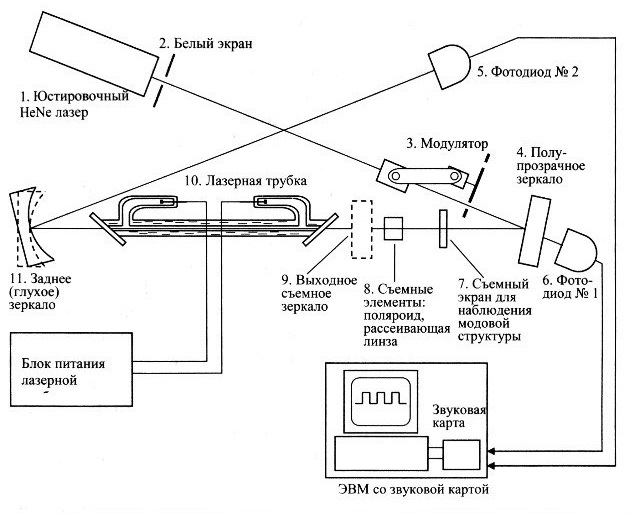
\includegraphics[width =  0.6\textwidth]{scheme}
			\caption{Схема экспериментальной установки. Штриховыми линиями показано положение зеркал при получении лазерной генерации на исследуемой трубке.}
			\label{scheme}
		\end{figure}
	
	Схема экспериментальной установки приведена на рис.\ref{scheme}. На одном оптическом рельсе расположены: головка промышленного He-Ne-лазера \CYRL \CYRG - 45 с исследуемой газоразрядной трубкой (11), заключённой в кожух (10), рейтер с полупрозрачным зеркалом (4), фотодиоды (5 и 6), а также 3 съёмных рейтера с выходным зеркалом (9), отрицательной линзой для наблюдения модовой структуры излучения исследуемого лазера или поляроидом для исследования поляризации выходного излучения лазера (8) и с белым экраном (7).
	
	Юстировочный лазер (1) с белым экранчиком (2) и модулятор (3) закреплены на втором оптическом рельсе. Модулятор может быть повёрнут в разные положения: при измерении коэффициента усиления он модулирует пучок, идущий от юстировочного лазера, при измерении поляризации излучения исследуемого лазера он модулирует выходящее из него излучение. В остальных случаях модулятор отводится в сторону, чтобы не перекрывать пучки.
	
	Юстировочный лазер предназначен для настройки положения всех элементов установки и является источником зондирующего излучения для измерения усиления активной среды исследуемого лазера.
	
	Зондирующий пучок сначала попадает на полупрозрачное зеркало (4). Часть излучения проходит сквозь зеркало и попадает на фотодиод №1 (6), с которого снимается сигнал, пропорциональный интенсивности зондирующего пучка. Отражённая часть направляется в исследуемую трубку.

	\newpage
	
	\section{Проведение измерений.}
	\subsection{Измерение усиления трубки.}
	
	Поведём по несколько раз измерения с включённым и выключенным питанием трубки для трёх значений тока через трубку. Данные занесём в таблицу \ref{t1}.
	
	\begin{table}[H]
		\centering
		\caption{Измерение коэффициента усиления трубки.}
		\label{t1}
			\resizebox{\textwidth}{!}{
				\begin{tabular}{c|c|c|c|cccc|c|c|ccc} \toprule
					$I,~\text{мА}$                & \multicolumn{3}{c|}{22} & \multicolumn{3}{c|}{30}                                                               & \multicolumn{3}{c|}{40} & \multicolumn{3}{c}{0}                                        \\ \midrule
					$U_{\text{эфф}_1},~\text{мВ}$ & 102.1  & 101.7  & 101.6 & \multicolumn{1}{c|}{102.5} & \multicolumn{1}{c|}{102.9} & \multicolumn{1}{c|}{103.4} & 103.4  & 103.4  & 104.1 & \multicolumn{1}{c|}{90.6} & \multicolumn{1}{c|}{91}   & 91.9 \\ \midrule
					$U_{\text{эфф}_2},~\text{мВ}$ & 79.7   & 79.3   & 79.2  & \multicolumn{1}{c|}{80.3}  & \multicolumn{1}{c|}{80.5}  & \multicolumn{1}{c|}{80.7}  & 80.5   & 80.6   & 80.8  & \multicolumn{1}{c|}{69.3} & \multicolumn{1}{c|}{69.3} & 70.3 \\ \bottomrule
				\end{tabular}
	}
	\end{table}

	\subsection{Поляризация излучения лазера.}
	
	Измерим зависимость интенсивности излучения исследуемого лазера от угла поворота поляроида. Данные занесём в таблицу \ref{t2}.
	
	\begin{table}[H]
		\centering
		\caption{Поляризация излучения лазера}
		\label{t2}
		\begin{tabular}{c|c|c|c|c|c|c|c|c|c|c} \toprule
			$\text{Угол поворота поляроида},~\degree$          & 0   & 20  & 40   & 60   & 80   & 100  & 120  & 140 & 160 & 180 \\ \midrule
			$U_\text{эфф},~\text{мкВ}$ & 306 & 580 & 1043 & 1486 & 1672 & 1520 & 1118 & 591 & 333 & 313 \\ \bottomrule
		\end{tabular}
	\end{table}
	
	\begin{table}[H]
		\centering
	
		\begin{tabular}{c|c|c|c|c|c|c|c|c|c} \toprule
			$\text{Угол поворота поляроида},~\degree$          & 200 & 220  & 240  & 260  & 280  & 300  & 320 & 340 & 360 \\ \midrule
			$U_\text{эфф},~\text{мкВ}$ & 617 & 1132 & 1412 & 1587 & 1394 & 1068 & 577 & 314 & 317 \\ \bottomrule
		\end{tabular}
	\end{table}

	\section{Обработка результатов.}
	
	По значениям эффективного напряжения в осциллограмме первого и второго каналов (с 1 и 2 фотодиодов соответственно) рассчитаем коэффициент усиления трубки. Обозначим за $U_{\text{эфф}_1}^0$ и $U_{\text{эфф}_2}^0$  показания программы при выключенной трубке, тогда $$\gamma = \dfrac{U_{\text{эфф}_2}}{U_{\text{эфф}_1}}/ \dfrac{U_{\text{эфф}_2}^0}{U_{\text{эфф}_1}^0}$$.
	
	Полученные результаты занесём в таблицу \ref{t3}.
	
	\begin{table}[H]
		\centering
		\caption{Коэффициент усиления трубки.}
		\label{t3}
		\begin{tabular}{c|c|c|c|c|c|c|ccc} \toprule
			$I,~\text{мА}$            & \multicolumn{3}{c|}{22}    & \multicolumn{3}{c|}{30}    & \multicolumn{3}{c}{40}                                          \\ \midrule
			$\gamma$             & 1.022   & 1.021   & 1.021  & 1.026   & 1.024   & 1.022  & \multicolumn{1}{c|}{1.019} & \multicolumn{1}{c|}{1.021} & 1.016 \\ \midrule
			$\gamma_\text{ср}$ & \multicolumn{3}{c|}{\textbf{1.021} $\pm$ 0.001} & \multicolumn{3}{c|}{\textbf{1.024} $\pm$ 0.001} & \multicolumn{3}{c}{\textbf{1.019} $\pm$ 0.002}   \\ \bottomrule                                   
		\end{tabular}
	\end{table}

Проанализируем зависимость интенсивности излучения исследуемого лазера от угла поворота поляроида. Для этого построим график зависимости отношения интенсивности излучения лазера к максимальной интенсивности от угла поворота поляроида. Данные возьмём из таблицы \ref{t3}. Необходимые для построения измерения занесём в таблицу \ref{t4}.

\begin{table}[H]
	\centering
	\caption{Поляризация излучения.}
	\label{t4}
	\begin{tabular}{c|c|c|c|c|c|c|c|c|c|c} \toprule
		$\text{Угол поворота поляроида},~\degree$ & 0    & 20   & 40   & 60   & 80   & 100  & 120  & 140  & 160 & 180  \\ \midrule
		$I/I_{max}$                               & 0.18 & 0.35 & 0.62 & 0.89 & 1.00 & 0.91 & 0.67 & 0.35 & 0.20 & 0.19 \\ \bottomrule
	\end{tabular}
\end{table}

\begin{table}[H]
	\centering
	\begin{tabular}{c|c|c|c|c|c|c|c|c|c} \toprule
		$\text{Угол поворота поляроида},~\degree$ & 200    & 220   & 240   & 260   & 280   & 300  & 320  & 340  & 360   \\ \midrule
		$I/I_{max}$                               & 0.37 & 0.68 & 0.84 & 0.95 & 0.83 & 0.64 & 0.35 & 0.19 & 0.19  \\ \bottomrule
	\end{tabular}
\end{table}
		
		\begin{figure}[H]
			\centering
			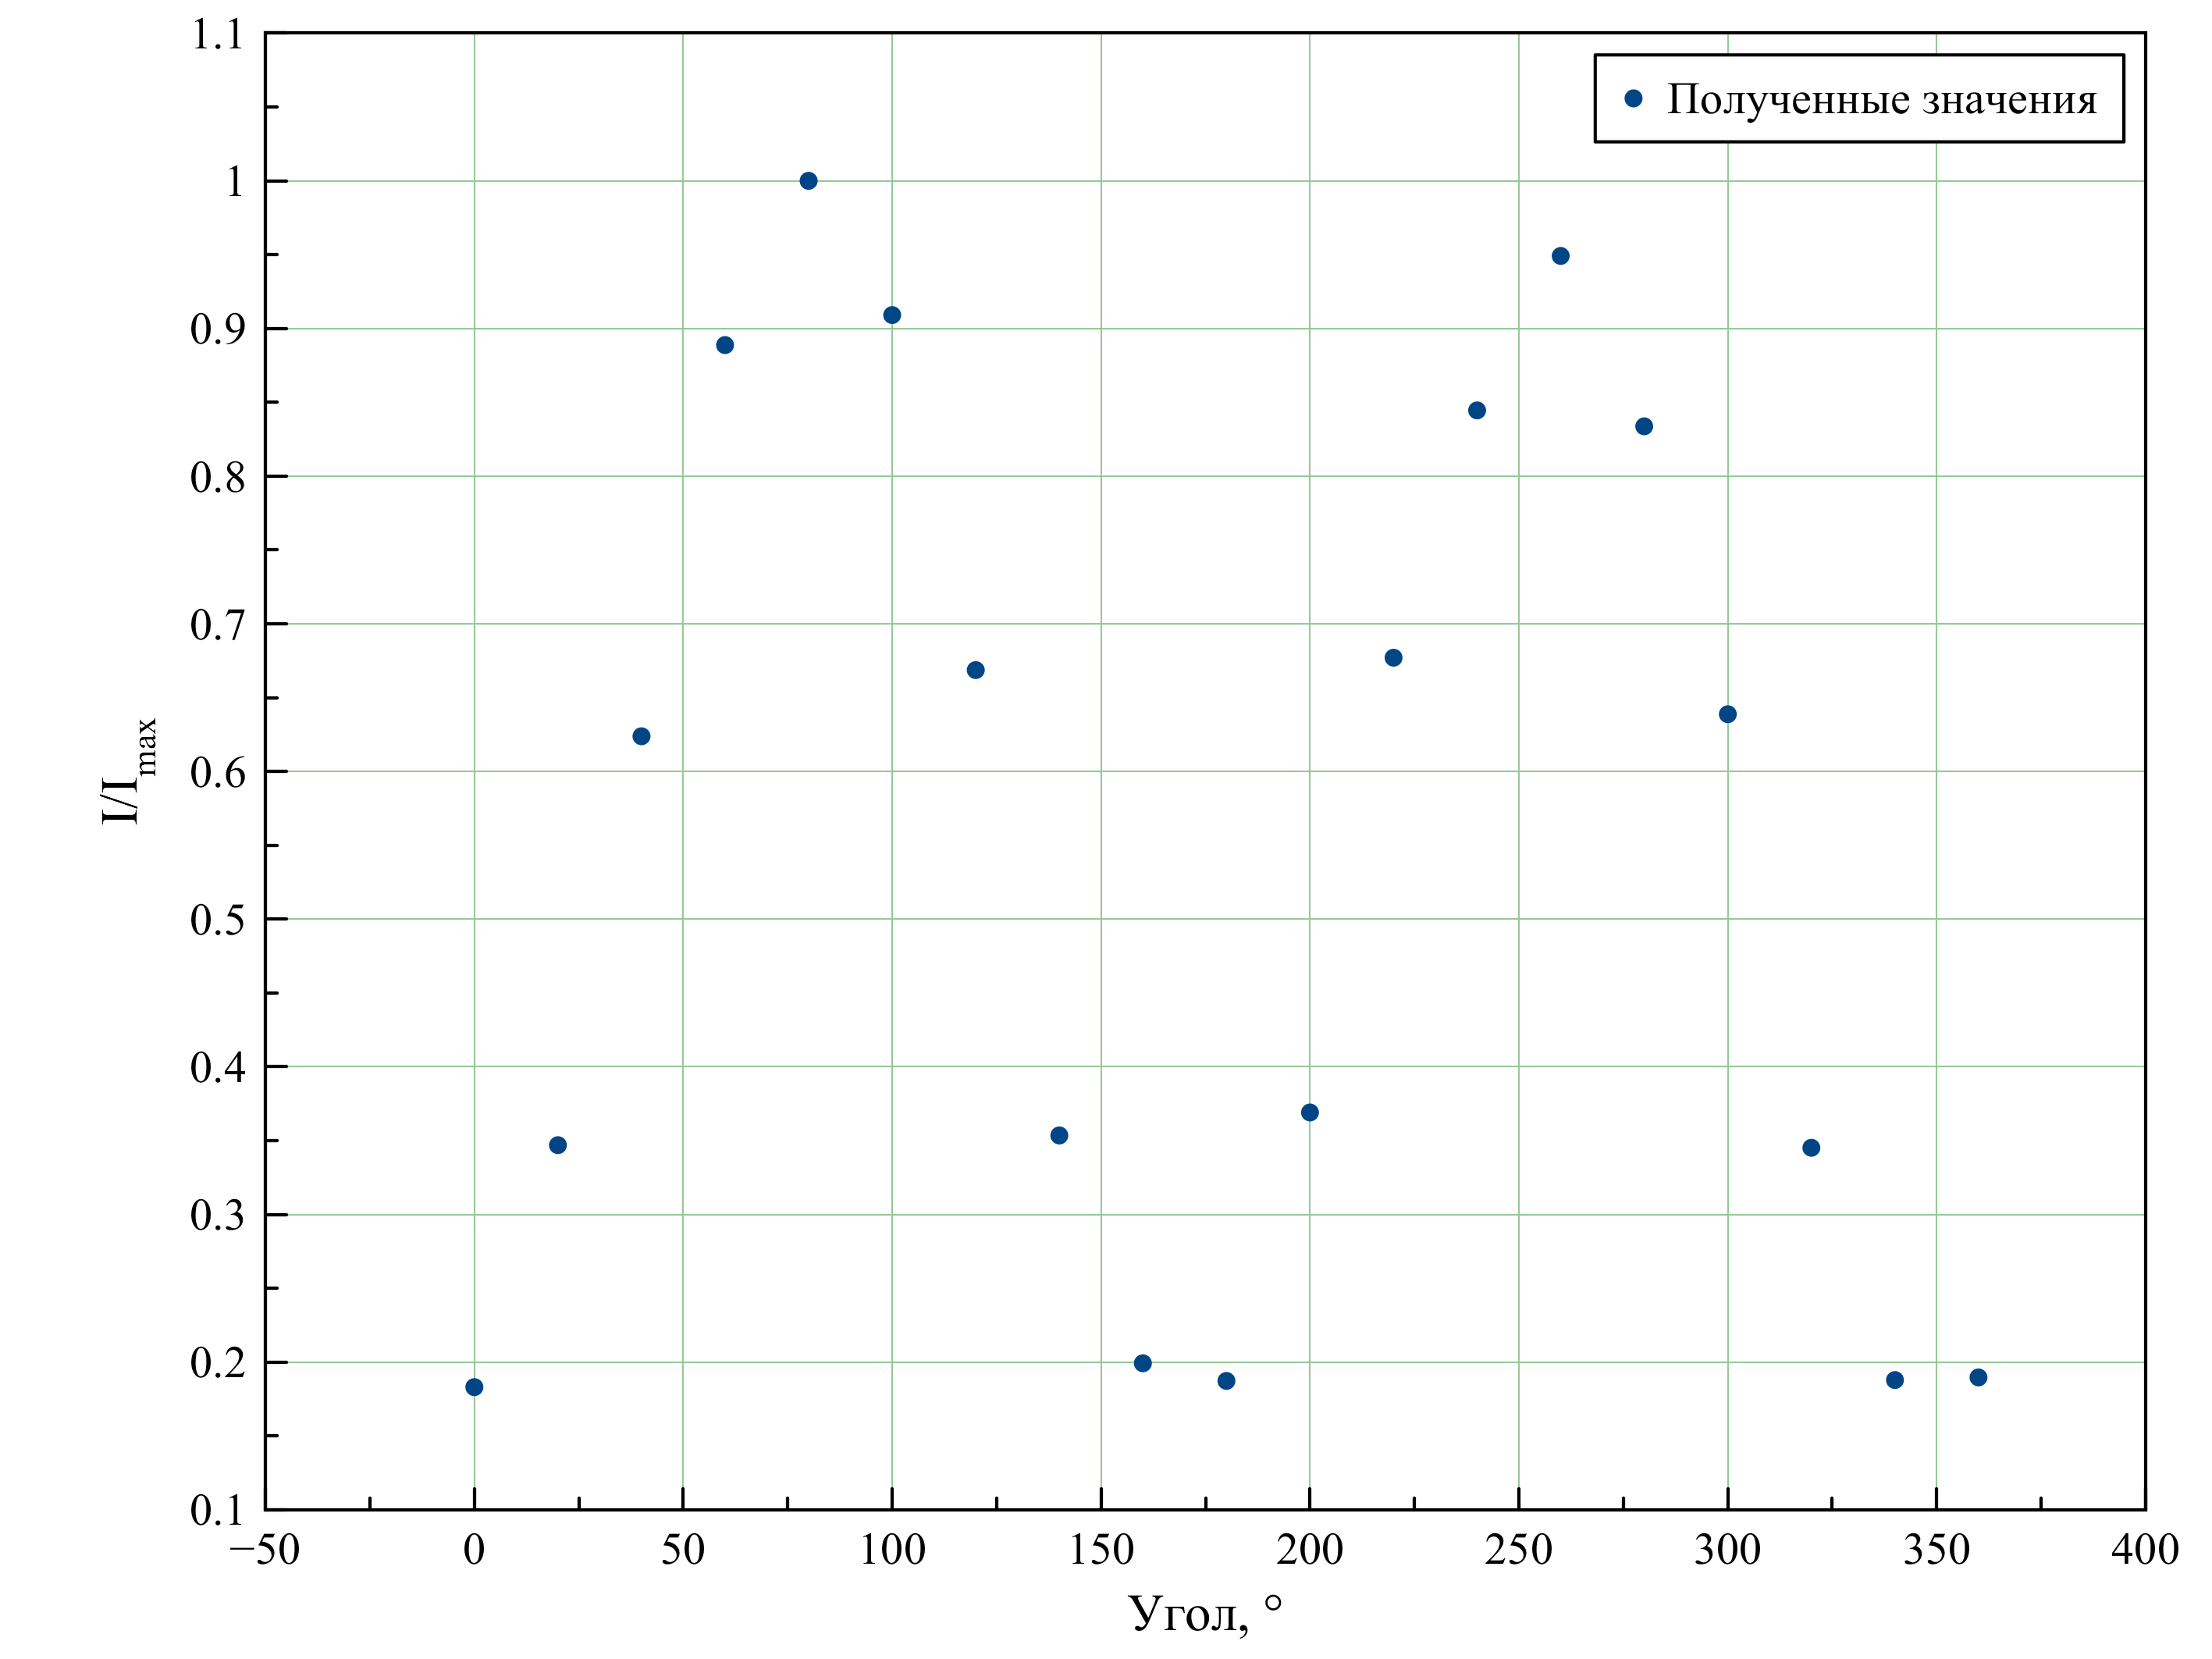
\includegraphics[width =  0.9\textwidth]{graph}
			\caption{Зависимость относительной интенсивности от угла поворота поляроида.}
			\label{graph}
		\end{figure}
	
	По полученной зависимости можно сказать, что излучение получилось линейно поляризованным.
	
	\section{Вывод.}
	\begin{itemize}
		\item В ходе лабораторной работы были изучены принципы работы гелий-неонового лазера, свойства лазерного излучения и измерено усиление лазерной трубки.
		
		\item Измеренной усиления полностью совпадает с теоретическим (характеристикой самой лазерной трубки) и составляет $1-3 \%$.
		
		\item Было проверено, что сгенерированное излучение линейно поляризовано.
		
		\item Было проведено наблюдение модовой структуры лазерного излучения, а именно, с помощью поворота выходного зеркала были получены одномодовый, трёхмодовый и многомодовый режимы.
	\end{itemize}

\end{document}